\documentclass[pdf]{beamer}
\usepackage{amsmath}
\usepackage{amsfonts}
\usepackage{amssymb}
\usepackage{bussproofs}
\usepackage{color}
\usepackage{lmodern}
\usepackage{listings}
\usepackage{natbib}
\usepackage{upgreek}
\usepackage{stmaryrd}
\usepackage{tikz}

\mode<presentation>{}

\newcommand{\T}[1]{\texttt{#1}}
\newsavebox{\codebox}
\newsavebox{\lengthbox}
\lstset{mathescape=true, basicstyle=\ttfamily}
\newcommand{\LP}{\langle}
\newcommand{\RP}{\rangle}
\newcommand{\LB}{\llbracket}
\newcommand{\RB}{\rrbracket}
\newcommand{\LL}{\langle\!\langle}
\newcommand{\RR}{\rangle\!\rangle}
\newcommand{\quadthree}{\qquad\quad}
\newcommand{\quadfour}{\quadthree\quad}
\newcommand{\quadfive}{\quadfour\quad}
\newcommand{\quadsix}{\quadfive\quad}
\newcommand{\quadseven}{\quadsix\quad}
\newcommand{\quadeight}{\quadseven\quad}
\newcommand{\quadten}{\quadfive\quadfive}

\title{Extracting Cost Recurrences from Sequential and Parallel Functional Programs}

\author{Justin Raymond}
\institute{Professor Norman Danner}

%\usecolortheme{fly}
%\setbeameroption{show notes}


\begin{document}
\begin{lrbox}{\codebox}
\begin{lstlisting}
rev = $\lambda$xs.rec(xs,
  Nil $\mapsto$ $\lambda$a.a,
  Cons$\mapsto \LP x,\LP xs,r \RP\RP.\lambda$a.force(r) Cons$\LP$x,a$\RP$))) Nil
\end{lstlisting}
\end{lrbox}

\defverbatim[colored]\lstfold{
  \begin{lstlisting}[language=Caml, xleftmargin=.2\textwidth, xrightmargin=.2\textwidth]
  fold f z xs =
    match xs with
      [] -> z
    | x::xs' -> f x (fold f z xs')
  \end{lstlisting}
}

\defverbatim[colored]\lstlength{
  \begin{lstlisting}[language=Caml, xleftmargin=.2\textwidth, xrightmargin=.2\textwidth]
  length xs =
    match xs with
      [] -> 0
    | (x::xs) -> 1 + length xs
  \end{lstlisting}
}

\defverbatim[colored]\lstfastreverse{
  \begin{lstlisting}[language=Caml, xleftmargin=.05\textwidth, xrightmargin=.05\textwidth]
  rev ys =
    let go xs =
      match xs with
        [] -> fun ys -> ys
      | (x::xs') -> fun a -> (go xs') (x::a)
    in go ys []

  rev xs = foldl (fun xs x -> x::xs) [] xs
  \end{lstlisting}
}

\defverbatim[colored]\lstinsert{
  \begin{lstlisting}[language=Caml, xleftmargin=.05\textwidth, xrightmargin=.05\textwidth]
  insert f y xs =
    match xs with
      [] -> [y]
    | x::xs' | f y x -> y::xs
    | x::xs' -> x::insert f y xs'
  \end{lstlisting}
}
\defverbatim[colored]\lstsort{
  \begin{lstlisting}[language=Caml, xleftmargin=.05\textwidth, xrightmargin=.05\textwidth]
  sort f xs =
    match xs with
      [] -> []
    | x::xs' -> insert f x (sort f xs')
  \end{lstlisting}
}
\defverbatim[colored]\lsttreemap{
  \begin{lstlisting}[language=Caml, xleftmargin=.05\textwidth, xrightmargin=.05\textwidth]
  map f t =
    match t with
      E -> E
    | N(x,l,r) -> N(f x, map f l, map f r)
  \end{lstlisting}
}

\begin{frame}
  \titlepage
\end{frame}

\begin{frame}{Overview}
  \begin{itemize}
    \item<1-> Complexity analysis aims to predict the resources, most often time and space, which a program requires
    \vfill
    \item<1-> Previous work by \citet{Danner2013} and \citet{Danner2015} formalizes the extraction of recurrences for the cost of higher-order functional programs
    \vfill
    \item<1-> Contribution:
      \begin{itemize}
          \item<1-> We use the method of \citet{Danner2015} to analyze the complexity of higher-order functional programs
          \vfill
          \item<1-> We extend the method to parallel cost semantics to help answer the question: how long will this program take to run on an arbitrary number of processors?
          \vfill
          \item<1-> We prove an interesting fact about the recurrences for the cost of programs
        \end{itemize}
  \end{itemize}
\end{frame}

\begin{frame}{Traditional Complexity Analysis}
  \begin{itemize}
    \item<1->[]Source program:
      \lstfold
      \vfill
    \item<1->[]Write down recurrence for cost:
      \[ T(n) = \begin{cases}
          c_0 &\text{ if } n = 0 \\
          c_1 + T(n-1) &\text{ otherwise}
        \end{cases}
      \]
      \vfill
    \item<1->[]Obtain a closed form solution:
      \[T(n) = c_1 n + c_1 = \mathcal{O}(n)\]

  \end{itemize}

  \note{\small
    Traditional complexity analysis of a recursive program, we write down a
    recurrence for the cost of the program. Then we solve the recurrence and drop
    the constant factors. There is no formal relation between the program and the
    recurrence.

    Traditional complexity analysis, you look at the program, you write down a
    recurrence which describes the cost, you solve the recurrence, you drop
    everything but the highest order term. There are drawbacks to this
    approach. The foremost is that there is no formal relationship between the
    source language program and the recurrence. This makes it easier to make
    mistakes. The second drawback is the traditional approach is not
    compositional. To analyze the composition of two functions $g \circ f$ we
    need to know something about the size of the result of $f$. This gets more
    complicated with higher order functions such as \T{fold}.

    Can we make this analysis higher-order? How do we take into account the
    asymptotic complexity of $f$?

    We could try to say that $f$ is $\mathcal{O}(x)$ where $x$ is the size of
    the sum of its arguments. But how big are the sum of the arguments to $f$?

    The size of the inputs to $f$ depend on the size of each element in the
    list and the size of recursive calls to \T{fold}.

    How to address this? Enter the \citet{Danner2015}.
  }
\end{frame}

\begin{frame}{Higher-Order Complexity Analysis}
  \begin{itemize}
    \item<1-> Write programs in a "source language"
    \vfill
    \item<1-> Translate the programs to a "complexity language"
    \vfill
    \item<1-> The translated programs are recurrences for the complexity of the source language program
    \vfill
    \item<1-> \textbf{complexity} = cost $\times$ potential
    \vfill
    \item<1-> \textbf{cost}: steps to run a program
    \vfill
    \item<1-> \textbf{potential}: size of the result of evaluating program
  \end{itemize}

\note{ \small
  \begin{itemize}
    \item How do analysis in a way that we have a formal connection between the
      program and the recurrence, is naturally higher-order, and compositional?

    \item Previous work by \citet{Danner2013} and \citet{Danner2015} developed
      a method to address this.
  \end{itemize}
}
\end{frame}

\begin{frame}{Source Language}
  \begin{itemize}
    \item Variant of System-T\\
      Types:
      \begin{align*}
        \tau &::= \T{unit}\ |\ \tau \times \tau\ |\ \tau \rightarrow \tau\ |\ \T{susp}\ \tau\ |\ \delta \\
      \end{align*}
      Expressions:
      \begin{align*}
        e ::=\ &x\ |\ \LP\RP\ |\ \lambda x.e\ |\ e\ e\ |\ \LP e,e\RP\ |\ \T{split}(e, x.x.e) \\
               &|\ \T{delay}(e)\ |\ \T{force}(e)|\ C^\delta\ e\ |\ \T{rec}^\delta(e, \overline{C \mapsto x.e_C}) \\
               &|\ \T{map}^\phi(x.v, v)\ |\ \T{let}(e, x.e)
      \end{align*}
    \vfill
    \item Programmer defined datatypes:
      \begin{center}
        \T{datatype list = Nil | Cons int$\times$list}
      \end{center}
  \end{itemize}

  \note{\small
    So what does the source language look like? It is a variant of System
    T. If you're like me and can never remember the differences between the
    variants on the lambda calculus, System T is the simply typed lambda
    calculus with primitive recursion. The source language as structural
    recursion as well as some additional mechanisms to control the cost of
    programs. So we have \T{let} expressions to avoid recomputation of values
    and suspensions to evaluating expressions we don't actually need.

    The source language also has programmer-defined datatypes. Here is an
    example of how you would define a list. The arguments to the constructor of
    a datatype must be strictly positive.
  }
\end{frame}

\begin{frame}{Source Language - Cost Semantics}
  \begin{itemize}
    \vfill
    \item Tuples:
      \begin{prooftree}
        \AxiomC{$e_0 \downarrow^{n_0} v_0$}
        \AxiomC{$e_1 \downarrow^{n_1} v_1$}
        \BinaryInfC{$\LP e_0, e_1 \RP \downarrow^{n_0 + n_1} \LP v_0, v_1 \RP$}
      \end{prooftree}
    \vfill
    \item Application:
      \begin{prooftree}
        \AxiomC{$e_0 \downarrow^{n_0} \lambda x.e_0'$}
        \AxiomC{$e_1 \downarrow^{n_1} v_1$}
        \AxiomC{$e_0'[v_1/x] \downarrow^n v$}
        \TrinaryInfC{$e_0\ e_1 \downarrow^{1 + n_0 + n_1 + n} v$}
      \end{prooftree}
    \vfill
    \item Structural Recursion:
      \tiny
      \begin{prooftree}
        \AxiomC{$e \downarrow^{n_0} C v_0$}
        \AxiomC{$\T{map}^{\phi_C}(y.\LP y, \T{delay}(rec(y, \overline{C \mapsto x.e_C}))\RP, v_0) \downarrow^{n_1} v_1$}
        \AxiomC{$e_C[v_1/x] \downarrow^{n_2} v$}
        \TrinaryInfC{$rec(e, \overline{C \mapsto x.e_C}) \downarrow^{1 + n_0 + n_1 + n_2} v$}
      \end{prooftree}
    \vfill
  \end{itemize}

  \note{\small
    \begin{itemize}
      \item Operational semantics  give meaning to a program by describing how
        individual steps in a computation take place

      \item Small step semantics: evaluation judgements describe single steps

      \item Big step semantics: describe how overall results obtained

      \item Cost semantics add costs to big step semantics. The judgments are
        of the form $e$ steps to $v$ in $n$ steps.
    \end{itemize}
  }
\end{frame}

\begin{frame}{Source Language}
  \begin{itemize}
    \vfill
    \item OCaml: \hfill\\
      \lstlength
    \vfill
    \item Source language:\hfill\\
      \vspace{10mm}
      $\lambda xs.\T{rec}(xs, \T{Nil}\mapsto 0, \T{Cons}\mapsto\LP x,\LP xs,r\RP\RP.1 + \T{force}(r))$
    \vfill
  \end{itemize}

  \note{\small
    As an example of what the source language program looks like. Here is a
    recursive function that computes the length of a list in OCaml and the same
    function in the source language. The \T{rec} construct gives us structural
    recursion. It evaluates an expression to a value, and based on the
    constructor of the value, evaluates to the appropriate branch. Inside the
    branch we are given access to the arguments to the constructor as well as a
    delayed computation representing the result of the recursive call.
  }
\end{frame}



\begin{frame}{Complexity Language}
  \begin{itemize}
    \item Types
      \begin{align*}
        T &::= \textbf{C} \ |\ \T{unit} \ |\ \Delta \ |\ T \times T \ |\ T \rightarrow T \\
        \textbf{C} &::= 0\ |\ 1\ |\ 2\ |\ ... \\
        \T{datatype}\Delta &= C^\Delta_0 \T{of} \Phi_{C_0}[\Delta] \ |\ ... \ |\ C^\Delta_{n-1} \T{of} \Phi_{C_{n-1}}[\Delta]
      \end{align*}
    \item Expressions
      \begin{align*}
        E &::= x\ |\ 0\ |\ 1\ |\ E + E\ |\ \LP\RP\ |\ \LP E,E \RP\ |\ \\
          &\quad \pi_0 E\ |\ \pi_1 E\ |\ \lambda x.E\ |\ E\ E\ |\ C^\delta\ E\ |\ \text{rec}^\Delta(E, \overline{C \mapsto x.E_C})
      \end{align*}
    \vfill
    \item No longer need mechanisms for controlling cost
  \end{itemize}

  \note{\small
    The complexity language is a language for recurrences for the cost and
    potential of a source language program. We add an additional type
    \textbf{C} for costs. The rest of the language is very similar to the
    source language except we no longer need the syntactic constructs for
    controlling the costs. So the complexity language does not have suspensions
    or let expressions.
  }
\end{frame}

\begin{frame}{Translation}
  \begin{itemize}
    \item Translate source language programs of type $\tau$ to complexity
      language programs of type $\textbf{C}\times \LL \tau \RR$
    \vfill
    \item \textbf{C} bound on the steps to evaluate the program
    \vfill
    \item $\LL\tau\RR$ expression for the size of the value
    \vfill
    \item Types of the translation function $\|\cdot\|$:
      \begin{align*}
        \|\tau\| &= \textbf{C} \times \LL \tau \RR \\
        \LL\T{unit}\RR &= \T{unit} \\
        \LL \sigma \times \tau \RR &= \LL \sigma \RR \times \LL \tau \RR \\
        \LL \sigma \rightarrow \tau \RR &= \LL \sigma \RR \rightarrow \|\tau\| \\
        \LL \T{susp}\ \tau \RR &= \|\tau\| \\
        \LL \delta \RR &= \delta \\
      \end{align*}
  \end{itemize}

  \note{\small
    The translation function cross compiles source language programs to
    complexity language programs. So a source language program of type $\tau$
    is translated to a complexity language program of type $\textbf{C}\times
    \LL \tau \RR$. The \textbf{C} component is a bound on the steps to evaluate
    the program and $\LL \tau \RR$ is a complexity language expression for the
    size of the result of executing the program.

    Abstractions are less straightforward. The cost of evaluating an
    abstraction is $0$, since abstractions are in normal form.  The potential
    of the translation of an abstraction is a function from potentials to
    complexities. Recall that a potential captures the cost of future uses of
    an expression. The cost of future uses of a function depends on the size of
    inputs you apply it to. So the potential of an abstraction is a function
    whose argument is a potential. Since applying a function has both a cost
    and a result. The codomain of the potential of the abstraction translation
    is a cost and a potential, aka a complexity.
}
\end{frame}

\begin{frame}{Translation}
   \begin{itemize}
    \item Some cases of the translation function:
    \item[]
      \begin{align*}
        \|x\| &= \LP 0,x \RP \\
        \|\LP e_0,e_1 \RP\| &= \LP \|e_0\|_c + \|e_1\|_c, \LP \|e_0\|_p,\|e_1\|_p\RP\RP \\
        \|\lambda x.e\| &= \LP 0, \lambda x.\|e\|\RP \\
        \|e_0\ e_1\| &= (1 + \|e_0\|_c + \|e_1\|_c) +_c \|e_0\|_p \|e_1\|_p \\
        %\|\T{delay}(e)\| &= \LP 0,\|e\| \RP \\
        %\|\T{force}(e)\| &= \|e\|_c +_c \|e\|_p
      \end{align*}
  \end{itemize}

  \note{\small
    Here are some cases of the translation function to get a better idea of
    what is going on. In the variable case, the result of the translation is
    $\LL 0,x \RR$. The cost of evaluating the variable is $0$ as it is already
    in normal form. The potential is the variable itself. The cost of
    translating a pair is the sum of the costs of translating the elements of
    the tuple. The potential is the pair of the potentials of the translations
    of the expressions.
  }
\end{frame}


\begin{frame}{Size-Based Denotational Semantics}
  \begin{itemize}
    \item Complexity translation does not lose any information
    \item Abstract values to their sizes using a denotational semantics
    \item \textbf{denotational semantics} - assign meanings to programs by
      interpreting types as sets and terms as elements of sets
    \item We use a standard denotational semantics
      %\begin{itemize}
      %  \item Numbers as natural numbers
      %  \item Tuples as cartesian products
      %  \item Abstractions as mathematical functions
      %\end{itemize}
    %\item Programmer-defined datatypes and \T{rec} non-standard
    \item Must define the following for programmer defined datatypes:
      \begin{itemize}
        \item $\LB \delta \RB$ - the set in which to interpret the type
        \item $D^\delta$ - sum type representing the unfolding of the datatype
        \item $size : D^\delta \to \LB \delta \RB$ - function from sum type to interpretation
      \end{itemize}
    \item The interpretation of the recursor is non-standard
      \[
        \LB rec(E, \overline{C \mapsto x.E_C}) \RB \xi = \bigvee\limits_{size(z) \leq \LB E \RB \xi} case(z, \overline{f_C})
      \]
  \end{itemize}

\note{\small
    The translation of a term to the complexity language does not throw
    away any information. That is, there is no abstractions about the list. To
    do so we interpret the complexity language expression in a denotational
    semantics. Denotational semantics assign meanings to programs by
    interpreting types as sets and terms as elements of the set corresponding
    to their type. Abstractions of type $\tau \to \sigma$ are interpreted as
    mathematical functions with domain $\tau$ and codomain $\sigma$. We use
    standard denotational semantics. The exception is programmer-defined
    datatypes. There are multiple interpretations of the size of a datatype.
    For example, if our natural numbers are fixed width integers we may want to
    interpret all natural numbers as having the same size. We may also
    interpret natural numbers as an inductively defined datatypes, where the
    interpretation of a natural number is the number itself. Another example is
}
\end{frame}


\begin{frame}{Fast Reverse - Specification and Implementation}
  \begin{itemize}
    \item
        $\T{datatype list} = \T{Nil of unit}\ |\ \T{Cons of int} \times \T{list}$
    \item
      Specification: \T{rev [$x_0,\dots,x_{n-1}$] = [$x_{n-1},\dots,x_0$]}
    \item[] Implementation:
      \lstfastreverse
    \item[]
      \usebox{\codebox}
  \end{itemize}

  \note{\small
    I'll go through two examples. The first is a higher-order function. The
    function reverses a list but uses a higher-order function to do so in linear
    time. Here is the implementation in OCaml. You'll notice that this is in fact a
    higher-order fold, and that we can write the function using a fold like so.
}
\end{frame}

\begin{frame}{Fast Reverse - Implementation}
  \begin{itemize}
    \vfill
    \item
      \T{rev (Cons$\LP$0,Cons$\LP$1, Nil$\RP\RP$)}
    \vfill
    \item
    \T{$\to_\beta$
      rec(Cons$\LP$0,Cons$\LP$1,Nil$\RP\RP$,
          Nil $\mapsto\lambda$a.a
          Cons$\mapsto \LP x,\LP xs,r\RP\RP.\lambda$a.force(r) Cons$\LP$x,a$\RP$) Nil}
    \vfill
    \item
      \T{$\to^*_\beta (\lambda$a0.($\lambda$a1.($\lambda$a2.a2) Cons$\LP$1,a1$\RP$) Cons$\LP$0,a0$\RP$) Nil}
    \vfill
    \item
      $\to_\beta$ ($\lambda$a1.($\lambda$a2.a2) Cons$\LP$1,a1$\RP$) Cons$\LP$0,Nil$\RP$
    \vfill
    \item
      $\to_\beta$ ($\lambda$a2.a2) Cons$\LP$1,Cons$\LP$0,Nil$\RP\RP$
    \vfill
    \item
      $\to_\beta$ Cons$\LP$1,Cons$\LP$0,Nil$\RP\RP$
    \vfill
  \end{itemize}

  \note{\small
    To give you an intuition into how this works, we the recursion results
    in nested functions. Each function takes a list of an argument and conses
    and element of to the list. The outermost function conses the first element
    of the original list and the innermost function conses the last element.
    Since the outermost function is evaluated first, the first element gets
    consed onto an empty list first and the last element gets consed on last,
    resulting in a reversed list. (DRAW PICTURE).
  }
\end{frame}

\begin{frame}{Fast Reverse - Translation}
  \small
  \begin{itemize}
    \item $\|\T{rev}\|$
      \begin{align*}
       &\LP 0, \lambda xs. 1 +_c \T{rec}(xs, \T{Nil} \mapsto \LP 1, \lambda a. \LP 0,a \RP\RP \\
      &\quad \T{Cons}\mapsto \LP x, \LP xs', r\RP\RP.\LP 1, \lambda a.(1 + r_c) +_c r_p\ \T{Cons}\LP \pi_1 x, a \RP\RP)\ \T{Nil}\RP\\
      \end{align*}
%    \item $\|\T{rev xs}\|$
%    \begin{align*}
%      &1 +_c (\lambda xs.\T{rec}(xs, \T{Nil} \mapsto \LP 1, \lambda a. \LP 0, a \RP \RP \\
%  &\quad \T{Cons}\mapsto \LP x, \LP xs', r\RP\RP. \LP 1, \lambda a.(1 + r_c) +_c r_p\ \T{Cons}\LP x, a \RP \RP)\ \T{Nil})\ xs
%    \end{align*}
  \end{itemize}

  \note{\small
    This is the result of the translation into the complexity language. The
    first term is the complexity of the function \T{rev} itself. The cost is
    $0$ and the potential is a function from potentials to complexities. We are
    interested in the analysis of applying the function \T{rev} to some list,
    so the translation of \T{rev xs} also shown.
  }
\end{frame}

\begin{frame}{Fast Reverse - Interpretation}
  We need to provide an interpretation for programmer-defined datatypes
  \begin{flalign*}
    \LB \T{list} \RB &= \mathbb{N}\\
    D^{list} &= \{\ast\} + \{1\} \times \mathbb{N}\\
    size_{list}(\ast) &= 1\\
    size_{list}(1,n) &= 1 + n\\
  \end{flalign*}

  \note{\small
    The translation of a term to the complexity language does not throw
    away any information. That is, there is no abstractions about the list. To
    do so we interpret the complexity language expression in a denotational
    semantics. Denotational semantics assign meanings to programs by
    interpreting types as sets and terms as elements of the set corresponding
    to their type. Abstractions of type $\tau \to \sigma$ are interpreted as
    mathematical functions with domain $\tau$ and codomain $\sigma$. We use
    standard denotational semantics. The exception is programmer-defined
    datatypes. There are multiple interpretations of the size of a datatype.
    For example, if our natural numbers are fixed width integers we may want to
    interpret all natural numbers as having the same size. We may also
    interpret natural numbers as an inductively defined datatypes, where the
    interpretation of a natural number is the number itself. Another example is
    trees. We may want to interpret trees as their number of nodes. We may also
    want to interpret trees as their number of nodes and the maximum size of
    their label. Another possible interpretation is the height of the tree.

    Here we interpret lists as their lengths. We need $D$ because we need to be
    able to branch on a datatype in the denotational semantics, so we introduce
    the sum type $D$ representing the unfolding of the constructors.
  }
\end{frame}

\begin{frame}{Fast Reverse - Interpretation}
  Interpretation of the helper function
  \begin{align*}
    g(n) &= \bigvee\limits_{size\ z \leq n} case(z, f_C, f_N) \\
  &\text{where} \\
    f_{Nil}(x) &= (1, \lambda a.(0, a)) \\
   f_{Cons}(b) &= (1, \lambda a. (1 + g_c(\pi_1 b)) +_c g_p(\pi_1 b)\ (a + 1))\\
  \end{align*}

  \note{\small
    The interpretation of a structural recursion is a maximum over a $case$
    expression.

    This is a recurrence for the function. We want the recurrence for the
    complexity of the function applied to some value.
  }
\end{frame}

\begin{frame}{Fast Reverse - Interpretation}
  \begin{itemize}
    \item Let $h(n, a) = g_p(n)\ a$.
    \item The recurrence for the cost:
      \begin{equation}
        h_c(n,a) = \begin{cases}
          0 & n = 0 \\
          2 + h_c(n-1,a+1) & n > 0
        \end{cases}
      \end{equation}
    \item$h_c(n,a) = 2n$
    \item The recurrence for the potential:
      \begin{equation}
        h_p(n,a) = \begin{cases}
          a & n = 0 \\
          h_p(n-1,a+1) & n > 0
        \end{cases}
      \end{equation}
    \item $h_p(n,a) = n + a$
  \end{itemize}

  \note{\small
    So we let $h$ be the result of applying $g$ to the interpretation of some
    list $a$. In order to make the analysis easier we break the complexity
    recurrence into a recurrence for the cost and a recurrence for the
    potential. Then we can solve the recurrences to get closed form solutions.
    So the conclusion is the cost is linear in the length of the list and the
    potential is the sum of the two lists.
  }
\end{frame}

\begin{frame}{Parametric Insertion Sort - Source Language Insert}
  \small
  \begin{itemize}
    \vfill
    \item \T{list} datatype: \hfill\\
      $\T{data list} = \T{Nil of unit | Cons of int $\times$ list}$
    \vfill
    \item Specification: \hfill\\
      $ \T{insert f x }[x_0,...,x_{n-1}] = [x_0,...,x_i, x, x_{i+1},....,x_{n-1}]$ where \T{f x x$_{i+1}$ = True}.
    \vfill
    \item OCaml:\hfill \\
      \lstinsert
    \vfill
    \item Source language: \hfill\\
      \begin{flalign*}
        \T{insert} &= \lambda f.\lambda x.\lambda xs.\T{rec}(xs, \T{Nil} \mapsto \T{Cons} \LP x, \T{Nil}\RP, &\\
                   &\qquad \T{Cons}\mapsto \LP y, \LP ys,r \RP\RP.\T{rec}(f\ x\ y, \T{True}\mapsto \T{Cons}\LP x,\T{Cons}\LP y,ys \RP\RP, &\\
                   &\qquad\quad \T{False}\mapsto \T{Cons}\LP y,\T{force}(r)\RP)) &
      \end{flalign*}
      \vfill
  \end{itemize}

  \note{\small
    The next example is parametric insertion sort. Sorts a list based on a
    comparison function. So to sort it in ascending order we pass $\leq$ as the
    comparison function and to sort it descending we pass $\geq$ as the
    comparison function.

    We define our datatype of lists the same as before. The insertion function
    takes a comparison function, an element, and a list of elements and inserts
    the element into its place in the list.

    Insert is given in the source language and in OCaml.
  }
\end{frame}

\begin{frame}{Parametric Insertion Sort - Source Language Sort}
  \small
  \begin{itemize}
    \vfill
    \item Specification:\hfill\\
      \T{sort f} $[x_0,...,x_{n-1}]$ = $[y_0,...,y_{n-1}]$ such that $\forall
      y_{i}, x_{i+1}.\T{f}\ y_{i}\ y_{i+1} = \T{True}$ and $[y_0,...,y_{n-1}]$
      is a sorted permutation of $[x_0,...,x_{n-1}]$
    \vfill
    \item OCaml:\hfill \\
      \lstsort
    \vfill
    \item Source language: \hfill \\
      \begin{flalign*}
        \T{sort} &= \lambda f.\lambda xs.\T{rec}(xs, \T{Nil} \mapsto \T{Nil}, &\\
                 &\qquad \T{Cons} \mapsto \LP y,\LP ys,r \RP\RP.\T{insert}\ f\ y\ \T{force}(r)) &
      \end{flalign*}
    \vfill
  \end{itemize}

  \note{\small
    The sorting function recurses on the list and inserts the head of the list
    into the recursively sorted tail of the list.
  }
\end{frame}

\begin{frame}{Parametric Insertion Sort - Complexity Language}
  \vfill
  \begin{align*}
    \|\T{insert}\| &= \LP 0, \lambda f. \LP 0, \lambda x.\LP 0,\lambda xs. \T{rec}(xs, \T{Nil} \mapsto \LP 1,\T{Cons}\LP x,\T{Nil}\RP\RP, \\
             &\quad\quad \T{Cons}\mapsto \LP y, \LP ys,r \RP\RP. (3 + (f\ x)_c) +_c \T{rec}(((f\ x)_p\ y)_p, \\
             &\quadten\T{True}\mapsto \LP 1, \T{Cons}\LP x,\T{Cons}\LP y,ys\RP\RP\RP, \\
             &\quadten\T{False}\mapsto \LP 1 + r_c, \T{Cons}\LP y,r_p\RP\RP)))
  \end{align*}
  \vfill
  \begin{align*}
    \|\T{sort}\| &= \LP 0, \lambda f.\LP 0,\lambda xs.\T{rec}(xs, \T{Nil} \mapsto 1 +_c \LP 0,\T{Nil}\RP, \\
               &\quad \T{Cons} \mapsto \LP y,\LP ys,r \RP\RP.(4 + r_c) +_c ((\|\T{insert}\|_p f)_p y)_p r_p)\RP\RP
  \end{align*}
  \vfill

  \note{\small
    Here is the translation of the two functions into the complexity language.
  }
\end{frame}

\begin{frame}{Parametric Insertion Sort - Denotational Semantics}
  We interpret lists as a pair of their largest element and their length.
  \begin{align*}
    \LB \T{list} \RB &= \mathbb{Z} \times \mathbb{N} \\
            D^{list} &= \{\ast\} + \mathbb{Z} \times \mathbb{N} \\
  size_{list} (\ast) &= (0,0) \\
size_{list} ((i,(j,n))) &= (max\{i,j\},1 + n)
  \end{align*}

  \note{\small
    This time we will interpret lists as a pair of their size and their largest
    element.
  }
\end{frame}

\begin{frame}{Parametric Insertion Sort - Insert Interpretation}
  \begin{itemize}
    \item[]
      \small
      \begin{align*}
      g(i,n) &= \bigvee\limits_{size(z) \leq (i,n)} case(z, f_{Nil}, f_{Cons}) \\
             &\text{where}\\
      f_{Nil}(\ast) &= (1, (i, 1)) \\
        f_{Cons}(j,m) &= (3 + ((f\ x)_p\ i)_c) +_c ((1, (max(x,j), 2 + m)) \\
                    &\quadthree \vee (1 + g_c(j,m), (max(j,\pi_0 r_p), 1 + \pi_1 g_p(j,m))))
      \end{align*}
    \item Closed form solution for the cost:
      \[g_c(i,n) \leq (4 + ((f\ x)_p\ i)_c n + 1\]
    \item Closed form solution for the potential:
      \[g_p(i,n) \leq (max\{x, i\}, n+1)\]
  \end{itemize}

  \note{\small
    So the interpretation of insert is this mess. But we can still find closed
    formed solutions for the cost and the potential.
  }
\end{frame}

\begin{frame}{Parametric Insertion Sort - Sort Interpretation}
  \begin{itemize}
    \item[]
      \small
      \begin{align*}
      g(i, n) &= \bigvee\limits_{size(z)\leq n} case(z, f_{Nil}, f_{Cons}) \\
      %
              &\text{where}\\
      f_{Nil} &= (1, (0,0)) \\
    f_{Cons} &= (5 + g_c(j,m) + (f\ i)_p\ j)_c g_p(j,m), (max\{i,j\},g_p(j,m) + 1))
      \end{align*}
  %cost depends on potential
    \item Closed form solution for potential:
      \[g_p(i,n) \leq (i, n)\]
    \item Closed form solution for the cost:
      \[g_c(i,n) \leq (3 + ((f\ i)_p\ i)_c n^2 + 5n + 1\]
  \end{itemize}

  \note{\tiny
    Similarly this is the result of interpreting sort. We use the
    interpretation of insert in the interpretation of sort.
  }
\end{frame}


\begin{frame}{Parallel Cost Semantics}
  \begin{itemize}
    \vfill
    \item We can reduce the running time of a program by allowing independent
      computations to be executed simultaneously
    \vfill
    \item Extent to which parallelism can be exploited is limited by the
      dependencies between subcomputations
    \vfill
    \item We add \textit{implicit binary fork-join} parallelism to the source language
    \vfill
    \item Analysis should not be tied to a number of processors
    \vfill
    \item Need a new measure of cost which reflects potential parallelism
      opportunities
    \vfill
  \end{itemize}
\end{frame}


\begin{frame}{Parallel Cost Semantics}
  \begin{itemize}
    \item<1> \textbf{Cost graphs}
      \[
        \mathcal{C} ::= 0\ |\  1\ |\  \mathcal{C} \oplus \mathcal{C}\ |\  \mathcal{C} \otimes \mathcal{C}
      \]

    \item<2>\textbf{0} graph
    \item<2>[]
      \begin{center}
      
\begin{tikzpicture}[main node/.style={circle,draw,font=\sffamily\tiny\bfseries}]
        \node[main node] (1) {Source \& Sink};
      \end{tikzpicture}
      \end{center}

    \item<3>\vspace{0mm} \textbf{1} graph
    \item<3>[]
      \vspace{-10mm}
      \begin{center}
      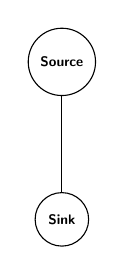
\begin{tikzpicture}[main node/.style={circle,draw,font=\sffamily\tiny\bfseries}, node distance=2cm]
        \node[main node] (1) {Source};
        \node[main node] (2) [below of=1] {Sink};
        \path[]
          (1) edge node [] {} (2);
      \end{tikzpicture}
    \end{center}

    \item<4> \vspace{-20mm} $G_0 \oplus G_1$:
      \begin{center}
        \vspace{-20mm}
        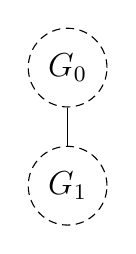
\begin{tikzpicture}%[main node/.style={circle,draw,font=\sffamily\Large\bfseries},node distance=3cm]
          \tikzstyle{main} = [circle, draw, font=\sffamily\tiny\bfseries, node distance=1.5cm]
          \tikzstyle{graph} = [circle, densely dashed,draw,minimum size=1cm,node distance=1.5cm]
        \node[graph] (1) [] {\large $G_0$};
        \node[graph] (2) [below of=1] {\large $G_1$};
        \begin{scope}
          \draw (1) -- (2);
        \end{scope}
      \end{tikzpicture}
    \end{center}

    \item<5> $G_0 \otimes G_1$:
      \begin{center}
        \vspace{-50mm}
        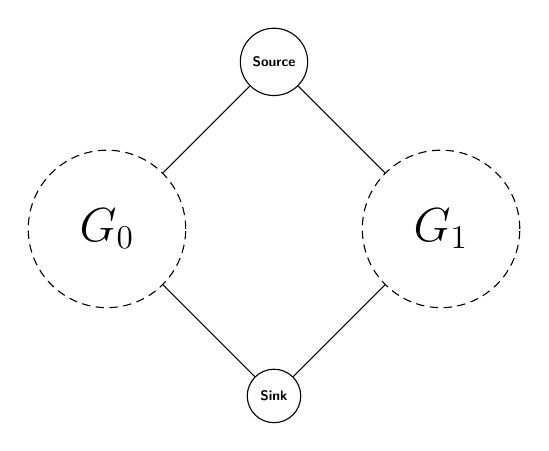
\begin{tikzpicture}%[main node/.style={circle,draw,font=\sffamily\Large\bfseries},node distance=3cm]
          \tikzstyle{main} = [circle, draw, font=\sffamily\tiny\bfseries, node distance=3cm]
          \tikzstyle{graph} = [circle, densely dashed,draw,minimum size=2cm,node distance=3cm]
        \node[main] (1) {Source};
        \node[graph] (3) [below left of=1] {\LARGE $G_0$};
        \node[graph] (4) [below right of=1] {\LARGE $G_1$};
        \node[main] (2) [below right of=3] {Sink};
        \begin{scope}
          \draw (1) -- (4);
          \draw (1) -- (3);
          \draw (4) -- (2);
          \draw (3) -- (2);
        \end{scope}
      \end{tikzpicture}
    \end{center}
  \end{itemize}

  \note{\small
    \begin{itemize}
      \item assign cost graph to the evaluation of an expression
      \item edges are sequentiality constraints
      \item source and sink reflect forking and joining overhead
    \end{itemize}
  }
\end{frame}

\begin{frame}{Parallel Cost Semantics}
  \begin{itemize}
    \item Assign cost graphs to the evaluation of expressions
      \vfill
      \begin{prooftree}
        \AxiomC{$e_0 \downarrow^{n_0} v_0$}
        \AxiomC{$e_1 \downarrow^{n_1} v_1$}
        \BinaryInfC{$\LP e_0, e_1 \RP \downarrow^{n_0 \otimes n_1} \LP v_0, v_1 \RP$}
      \end{prooftree}
      \vfill
      \begin{prooftree}
        \AxiomC{$e_0 \downarrow^{n_0} \lambda x.e_0'$}
        \AxiomC{$e_1 \downarrow^{n_1} v_1$}
        \AxiomC{$e_0'[v_1/x] \downarrow^n v$}
        \TrinaryInfC{$e_0\ e_1 \downarrow^{(n_0 \otimes n_1) \oplus n \oplus 1} v$}
      \end{prooftree}
      \vfill
  \end{itemize}

  \note{\small
    The second part of the thesis was demonstrating the flexibility of the
    technique by changing the cost model from number of steps (a natural
    number) to a cost graph. In the sequential model we charged for application
    and recursion. This gives a good estimate on the cost to execute a program
    that is run on one processor, but it does not give us any information on
    how the running time of the program will change if we scale to an arbitrary
    number of processors.

    So to address this, we introduce a new notion of cost. Instead of natural
    numbers, a cost is a cost graph. A cost graph is inductively defined as 0
    or 1 or c $\oplus$ c or c $\otimes$ c. A cost graph is an acyclic graph with a source node and a sink node.

  }
\end{frame}

\begin{frame}{Parallel Complexity Translation}
  \vfill
  \begin{align*}
    \|\LP e_0, e_1 \RP \| &= \LP \|e_0\|_c \otimes \|e_1\|_c, \LP \|e_0\|_p, \|e_1\|_p\RP\RP \\
    \|\lambda x.e\| &= \LP 0, \lambda x.\|e\| \RP \\
    \|e_0\ e_1\| &= 1 \oplus (\|e_0\|_c \otimes \|e_1\|_c) \oplus_c \|e_0\|_p\ \|e_1\|_p \\
    \|delay(e)\| &= \LP 0, \|e\|\RP \\
    \|force(e)\| &= \|e\|_c \oplus_c \|e\|_p
  \end{align*}
  \vfill
  \textbf{Bounding Theorem:}
    If $\gamma \vdash e : \tau$, then $e \sqsubseteq_\tau \|e\|$\\
  \textit{proof:} by logical relations.
  \vfill
\end{frame}

\begin{frame}{Work and Span}
  \begin{itemize}
    \item \textbf{Work} total steps to run program
      \begin{equation*}
        work(c) = \begin{cases}
          0 &\text{if } c = 0 \\
          1 &\text{if } c = 1 \\
          work(c_0) + work(c_1) &\text{if } c = c_0 \oplus c_1 \\
          work(c_0) + work(c_1) &\text{if } c = c_0 \otimes c_1
        \end{cases}
      \end{equation*}
    \item \textbf{Span} critical path of program
      \begin{equation*}
        span(c) = \begin{cases}
          0 &\text{if } c = 0 \\
          1 &\text{if } c = 1 \\
          span(c_0) + span(c_1) &\text{if } c = c_0 \oplus c_1 \\
          max(span(c_0), span(c_1)) &\text{if } c = c_0 \otimes c_1
        \end{cases}
      \end{equation*}
  \end{itemize}
\end{frame}

\begin{frame}{Brent's Theorem}
  \begin{itemize}
    \item A program with work $w$ and span $s$ may be evaluated on $p$
      processors in $O(max(w/p,s))$ steps.
  \end{itemize}
\end{frame}

\begin{frame}{Parallel Tree Map}
  \begin{itemize}
    \item Tree definition:
      \[ \T{datatype tree} = \T{E of Unit | N of int$\times$tree$\times$tree} \]
    \item OCaml:
      \lsttreemap

    \item Source Language:
      \begin{align*}
        \T{map} &= \lambda f.\lambda t.\T{rec}(t, \T{E} \mapsto \T{E}, \\
                &\qquad \T{N} \mapsto \LP x, \LP t_0, r_0 \RP, \LP t_1, r_1 \RP\RP.\T{N} \LP f\ x, \T{force}(r_0), \T{force}(r_1)\RP)
      \end{align*}
  \end{itemize}
\end{frame}

\begin{frame}{Parallel Tree Map}
  \begin{itemize}
      \vfill
    \item Translation:
      \begin{align*}
      \|\T{map}\| &= \LP 0.\lambda f.\LP 0,\lambda t.\T{rec}(t_p, \T{E} \mapsto \LP 1, \T{E}\RP, \\
  &\quadfour \T{N} \mapsto \LP y, \LP t_0, r_0 \RP \LP t_1, r_1 \RP \RP.  \\
  &\quadsix \LP 2 \oplus (f\ x)_c \otimes r_{0c} \otimes r_{1c}, \T{N} \LP (f\ x)_p, r_{0p}, r_{1p}\RP\RP
      \end{align*}
      \vfill
  \end{itemize}
\end{frame}

\begin{frame}{Parallel Tree Map}
  \begin{itemize}
      \vfill
    \item Interpret trees as largest label and number of nodes:
      \begin{align*}
        \LB tree \RB &= \mathbb{Z} \times \mathbb{Z} \\
        D_\T{tree} &= \{\ast\} + \mathbb{Z} \times \LB \T{tree} \RB \times \LB \T{tree} \RB \\
        size_\T{tree}(\ast) &= (0, 0) \\
        size_\T{tree}(x, (m_0, n_0), (m_1, n_1)) &= (max(x, m_0, m_1), 1 + n_0 + n_1)
      \end{align*}
      \vfill
    \item Interpret cost graphs as work and span:
      \begin{align*}
        \LB 0 \RB\xi &= (0,0) \\
        \LB 1 \RB\xi &= (1,1) \\
        \LB c_0 \oplus c_1 \RB\xi &= (\LB c_0 \RB\xi + \LB c_1 \RB\xi, \LB c_0 \RB\xi + \LB c_0 \RB \xi)\\
        \LB c_0 \otimes c_1 \RB\xi &= (\LB c_0 \RB\xi + \LB c_1 \RB\xi, max(\LB c_0 \RB\xi, \LB c_1 \RB\xi))
      \end{align*}
      \vfill
  \end{itemize}
\end{frame}

\begin{frame}{Parallel Tree Map}
  \begin{itemize}
    \item
      \footnotesize
\begin{align*}
  g(i,n) &= \bigvee\limits_{size(z) \leq (i,n)} case(z, f_E, f_N)
\end{align*}
where
\begin{align*}
  f_E(\ast) &= \LB \LP 1, \T{E} \RP\RB\xi = ((1, 1), (0, 0)) \\
  f_N(j, (j_0,n_0), (j_1, n_1)) &= \LB \LP 2 \oplus (f_p\ x)_c \otimes r_{0c} \otimes r_{1c}, \T{N} \LP (f_p\ x)_p, r_{0p}, r_{1p}\RP\RP \RB\\
                                &\quad \{t \mapsto (i,n), f \mapsto f, x \mapsto j, r_0 \mapsto g(j_0,n_0), r_1 \mapsto g(j_1,n_1) \} \\
                                &= ((2 + (f_p\ j)_c + \pi_0g_c(j_0,n_0) +\pi_0 g_c(j_1,n_1), \\
                                &\quadfour 2 + max((f_p\ j)_c,\pi_1 g_c(j_0,n_0), \pi_1 g_c(j_1,n_1))),\\
                                &\quadthree (max((f_p\ i)_p, \pi_0 g_p(j_0,n_0), \pi_1 g_p(j_1,n_1)), \\
                                &\quadfour 1 + \pi_1 g_p(i_0,n_0) + \pi_1 g_p(i_1,n_1)))
\end{align*}
  \end{itemize}
\end{frame}

\begin{frame}{Parallel Tree Map}
  \begin{itemize}
    \vfill
    \item Work:\hfill \\
      \[\pi_0 g_c(i,n) = (3 + (f\ i)_c)n + 1\]
    \vfill
    \item Span:\hfill \\
      \[\pi_1 g_c(i,n) \leq 2 + (f\ i)_c + n\]
    \vfill
    \item Brent's Theorem:\hfill \\
      \[ \mathcal{O}(max\left(\frac{(f\ i)_c n}{p}, (f\ i)_c + n\right)) \]
  \end{itemize}

  \note{\small
    \begin{itemize}
      \item asymptotic bound on the time  complexity
    \end{itemize}
  }
\end{frame}

\begin{frame}{Mutual Recurrences}
  \vfill
  Pure Potential Translation
    \begin{align*}
      |\LP e_0, e_1 \RP | &= \LP |e_0|, |e_1| \RP                                  \\
      |\lambda x.e | &= \lambda x.|e|                                                              \\
      |e_0\ e_1| &= |e_0|\ |e_1|                                                                   \\
      |delay(e)| &= |e|                                                                            \\
      |force(e)| &= |e|
    \end{align*}
  \vfill
  \textbf{Theorem:}
    For all $\gamma \vdash e : \tau$, $|e| : \LL \tau \RR \sim_\tau \|e\| : \|\tau\|$\\
  \textit{proof}: by logical relations
  \vfill
\end{frame}


\begin{frame}{Bibliography}
  \bibliography{bibliography}
  \bibliographystyle{plainnat}
\end{frame}

\end{document}
